En esta secci\'on se presentan algunos \'arboles de derivaci\'on de cadenas v\'alidas para la gram\'atica presentada.\\

\subsection{Ejemplo 1 - Aritm\'etico}
El siguiente ej\'emplo corresponde a la cadena:\\
$+N / (N-N*N*-N)$
Lo interesante de esta cadena es ver que no genera ambiguedades con el uso de los signos para los n\'umeros.
\begin{figure}[!h]
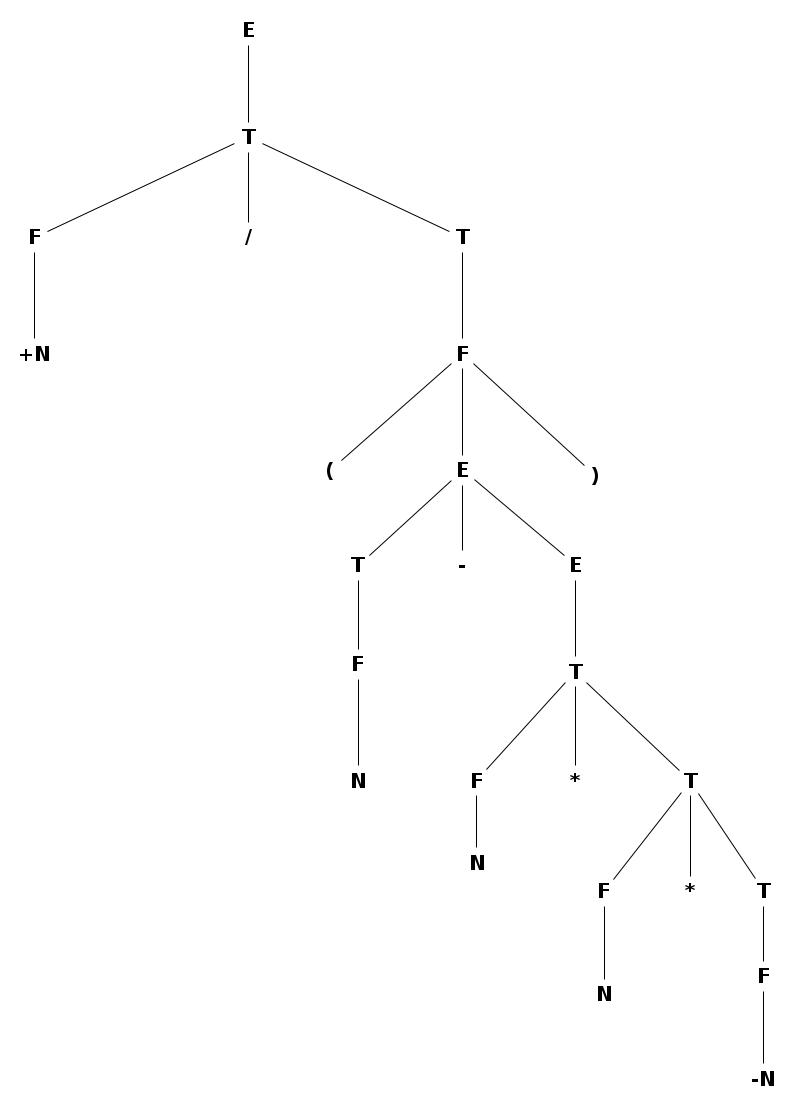
\includegraphics[scale=0.40]{arboles_derivacion/ejemplo1.jpg}
\end{figure}
\subsection{Ejemplo 2 - Aritm\'etico}
El ej\'emplo 2 se corresponde a la cadena:
$N*N+N*N$
\centerline{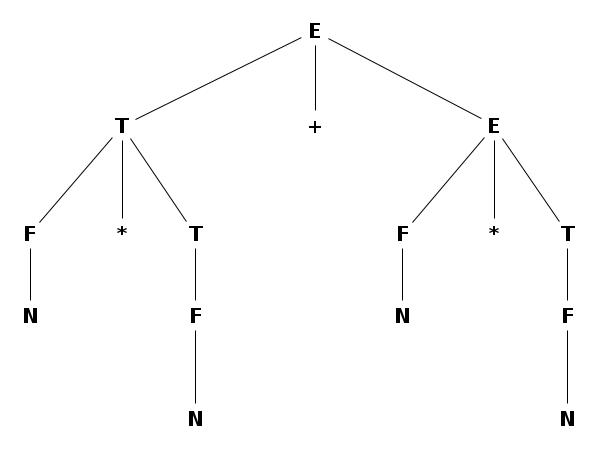
\includegraphics[scale=0.40]{arboles_derivacion/ejemplo2.jpg}}


\subsection{Ejemplo 3 - Programa v\'alido}

\centerline{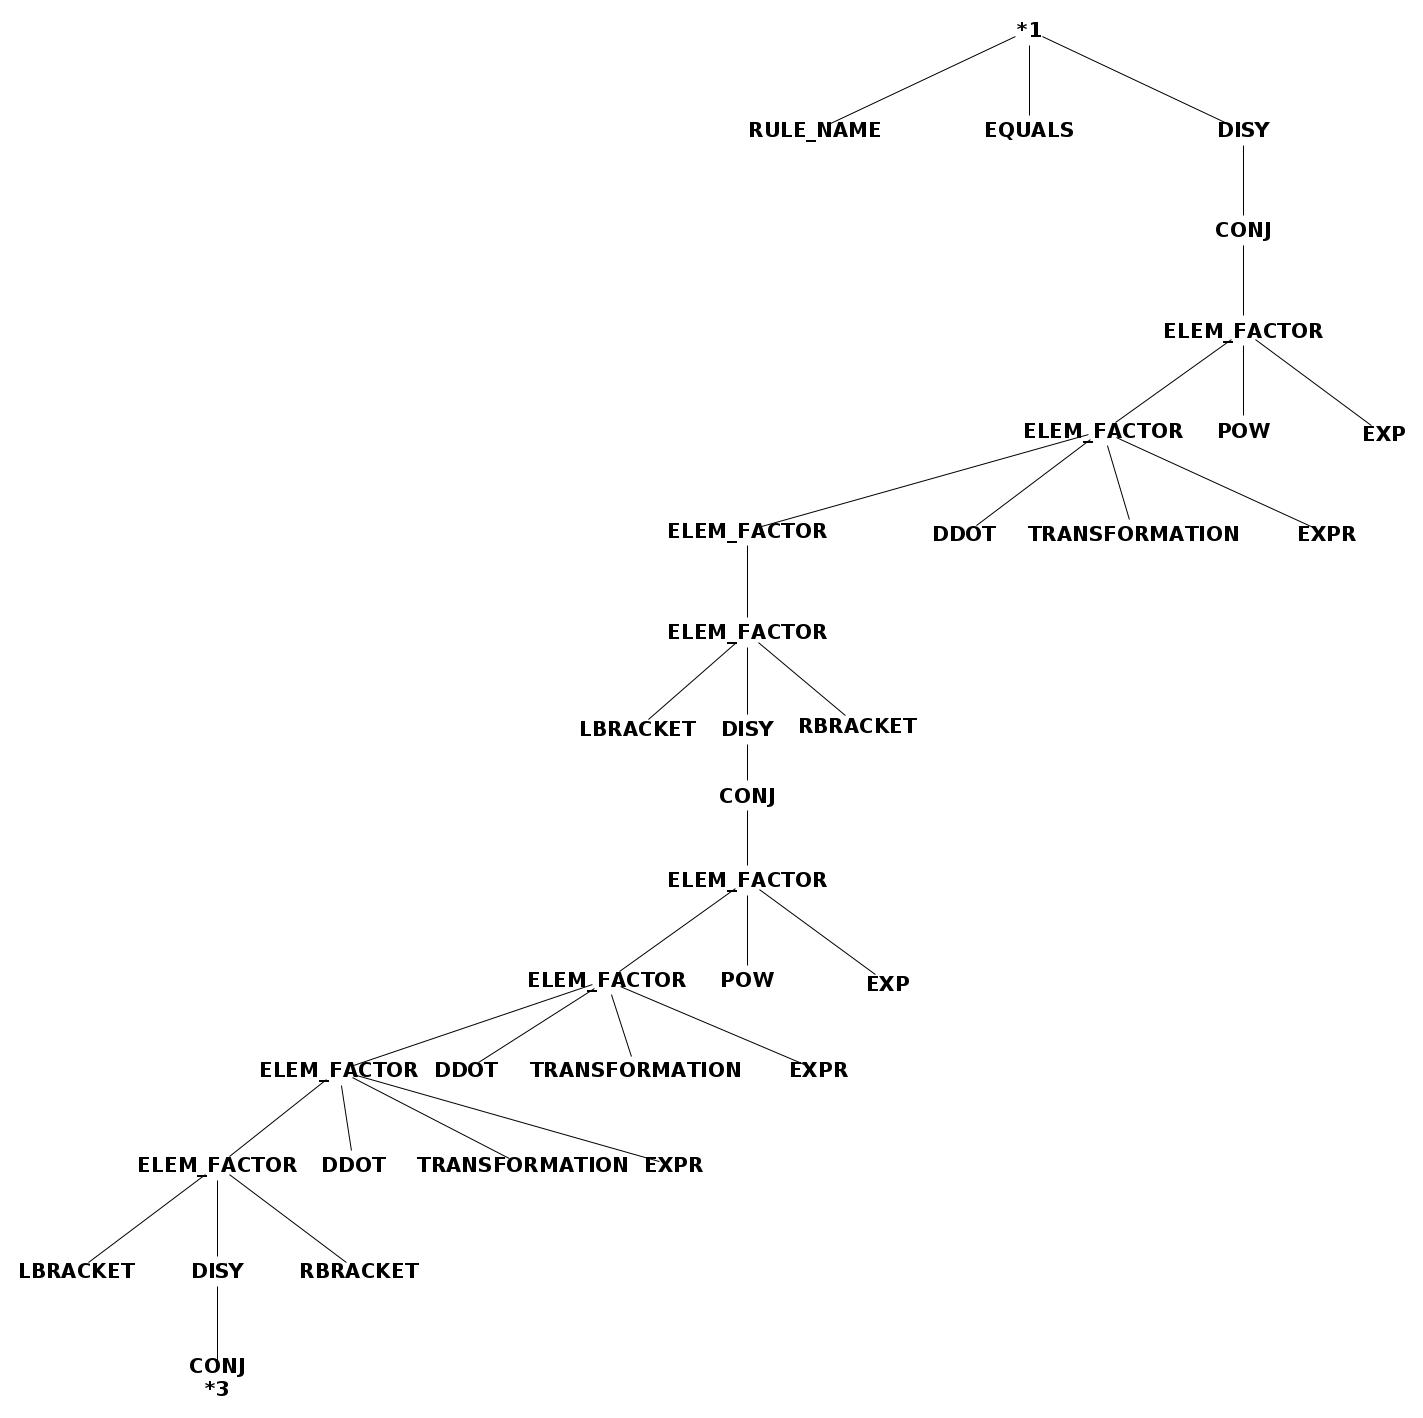
\includegraphics[scale=0.40]{arboles_derivacion/cube1.jpg}}


\subsection{Ejemplo 4 - Programa v\'alido}

\centerline{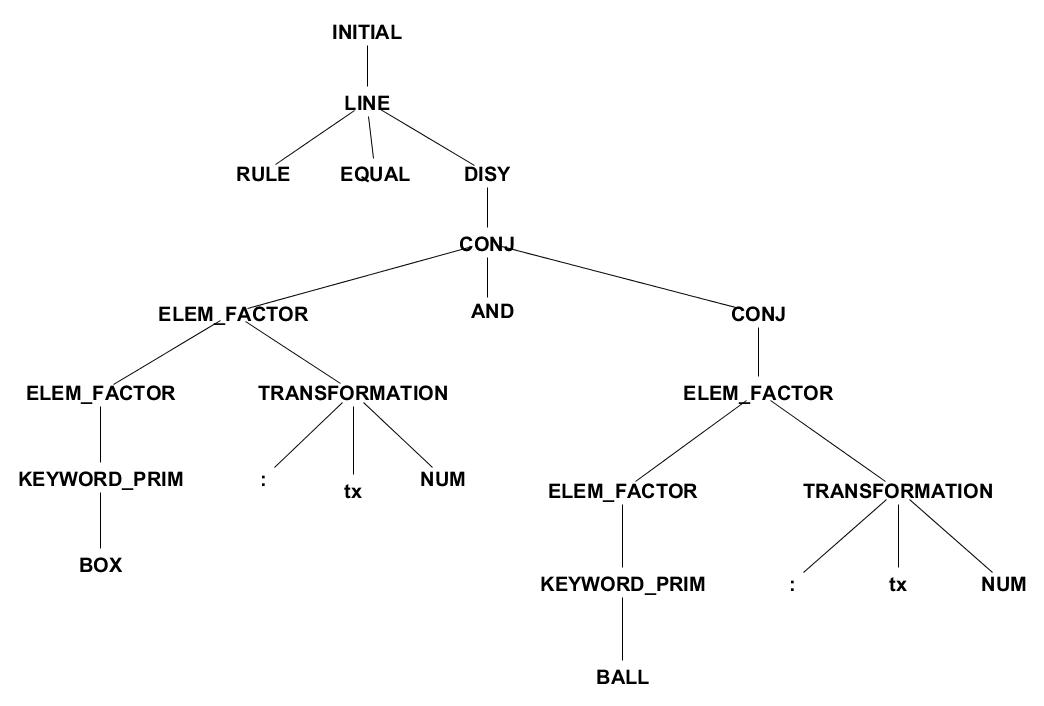
\includegraphics[scale=0.40]{arboles_derivacion/Ejemplo_and1.jpg}}

\subsection{Ejemplo 5 - Programa v\'alido}

\centerline{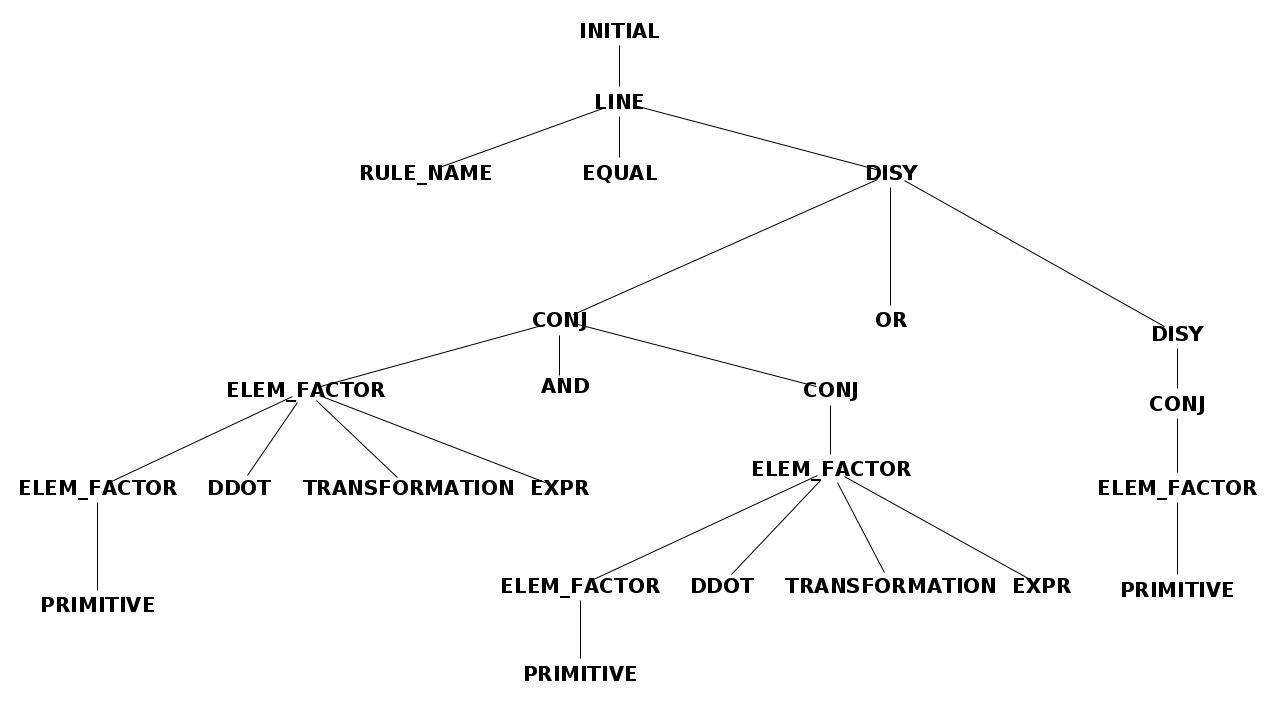
\includegraphics[scale=0.40]{arboles_derivacion/Ejemplo_and_or1.jpg}}
